\documentclass{article}
\usepackage{float}
\usepackage{graphicx}
\graphicspath{ {./} }

\title{Calculator -- User guide}
\date{}

\begin{document}
	\maketitle
	
	\tableofcontents
	
	\newpage
	
	\section{Introduction}
	This document is a user manual for our IVS project calculator.\\
	The purpose of this document is to provide the user with information on how to install and run the software as well as provide information about its use and functionality.\\
	The calculator is designed for the Ubuntu 64bit operating system.
	\newpage
	
	\section{Installation}
	\subsection{Installer}
	In order to install the calculator, firstly it is necessary to download the deb-package from our github repository at https://github.com/Jakub-Miko/IVS\_Kalkulacka.git. Once there, in the releases section you will find the downloadable debpackages. To instll the calculator choose the package ending with E-Calculator. Once you've chosen a release version you wish to use and downloaded the debpackage for it, all that's left is to run the following shell command: \\sudo apt\ install\ [DEBPACKAGE\_FILE\_NAME].\\
	In summary:
	\begin{itemize}
		\item{Visit https://github.com/Jakub-Miko/IVS\_Kalkulacka.git}
		\item{From the Releases section download desired package}
		\item{Once downloaded, run sudo apt\ install\ [DEBPACKAGE\_NAME]}
	\end{itemize}
	You can uninstall the calculator at any time by running the following shell command:\\
	sudo apt remove ivs-calculator-e-calculator 
	\\[5pt]
	To install the stddev utility use the package ending with -Profiler and uninstall with: sudo apt remove ivs-calculator-profiler
	\subsection{Manual Install}
	For the manual installation of the program it is necessary to have git installed, in order to clone the repository locally. To install git run:\\
	sudo apt install git\\
	After that run:\\
	git clone https://github.com/Jakub-Miko/IVS\_Kalkulacka.git\\
	Once cloned you need to go to IVS\_Kalkulacka/src and from there run the following command:\\
	sudo make install\\
	In order to uninstall the program manually again you need to be in IVS\_Kalkulacka/src and from there run the following:\\
	sudo make uninstall\\
	The stddev utility is installed this way by default.
	\newpage
	
	\section{Use}
	The calculator application is split into several segments:
	\begin{itemize}
		\item{Input field; here your inputs are displayed.}
		\item{Accumulator; in this section the results of your previous operations are stored.}
		\item{Numeric keyboard; by clicking on the buttons in this section you store the value of the button into the input field.}
		\item{Modular functions block; in this block the buttons are shared by the several sets of functions; you can swap between them by pressing the mod button at the top.}
		\item{Settings menu; this is stored at the top of the window and let's you change the sound effect settings.}
	\end{itemize}
	\begin{figure}[H]
		\centering
		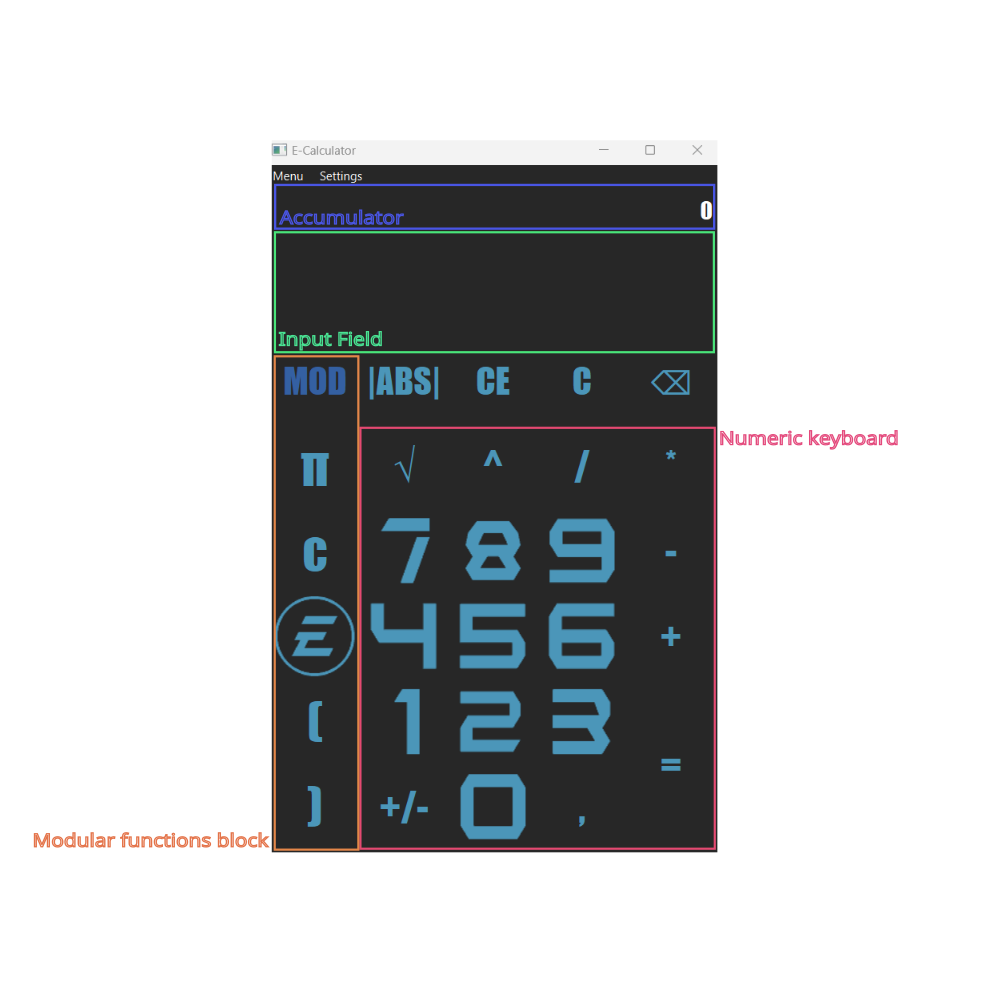
\includegraphics[width=0.8\textwidth]{kalkulacka_comment.png}
		\caption{Layout}
		\label{fig:enter-label}
	\end{figure}
	
	\subsection{Binary operations}
	The first input is expected to be a number, followed by the operation symbol and then a second number.
	
	In both cases upon entering another operation symbol the result of the previous equation is calculated, stored in the accumulator and then used as the first operand for the new operation.
	
	The Root operation works in the same way as any other binary function, where the first operand is the exponent and the second operand is the coefficient. 
	
	\subsection{Unary operations}
	All unary operations must by used after the argument and will immediately calculate the result as if you had pressed equals with a binary operation. if no value has been typed in beforehand, the operation will be performed on the result value in the currently opened parenthesis.
	
	\subsection{Parenthesis}
	The calculator also provides parenthesis. Opening a parenthesis saves the accumulator value and ongoing operation then begins a new one. Closing it calculates the result of the new expression within the parenthesis and finishes the saved operation, by passing it the result of the new parenthesis as an argument. By pressing the equals sign, all open parenthesis are closed and the final result is calculated.
	
	Note that this is not a parsing calculator so the result within the parenthesis is calculated as you type, and as such no operator precedence applies.
	
	\subsection{Rounding}
	Some operations like factorial, root and power only take some arguments as integers.
	If a non integer argument is passed a warning will be shown and the operation will proceed with a rounded value. Note that if the result is close enough to an integer, it may be considered a floating point error, and the error message will be suppressed.\\
	
\end{document}